\documentclass[11pt]{article}
\usepackage[utf8]{inputenc}
\usepackage[T1]{fontenc}
\usepackage{amsmath,amssymb,amsthm}
\usepackage[margin=1.1in]{geometry}
\usepackage{graphicx}
\usepackage{listings}
\usepackage{hyperref}
\lstset{basicstyle=\ttfamily\small,columns=fullflexible}
\emergencystretch=1em

\newtheorem{theorem}{Theorem}
\newtheorem{lemma}[theorem]{Lemma}
\newtheorem{remark}[theorem]{Remark}

\title{\texttt{w2filter}: a certified exhaustive streaming filter\\
for graphs with prescribed cycle spectrum}
\author{Antonio Guastella\\[2pt]
{\small\texttt{antonioguastella99@gmail.com}}}
\date{July 25, 2026}

\begin{document}
\maketitle

\begin{abstract}
We describe \texttt{w2filter}, a small ($\approx 420$ lines of C)
exhaustive streaming filter for the \texttt{graph6} output of
McKay's \texttt{nauty/geng}. Given a prescribed set $W$ of allowed
cycle lengths and a set $P$ of allowed path lengths, the filter
selects the graphs whose cycle spectrum is contained in $W$, checks
$2$-degeneracy and then classifies the \emph{graftable pairs}: pairs
$(u,v)$ such that \emph{every} simple $u$--$v$ path has length in
$P$. Every pruning step carries an explicit, human-checked
correctness proof shipped with the source, including proven bounds
for all DFS stacks; correctness is further
supported by an independent reference implementation, fixed anchor
classes with known census values and sanitizer-clean builds. On a
single core of a commodity desktop the filter alone sustains
$\approx 2\times 10^6$ graphs/second, so the full pipeline runs at
the speed of the \texttt{geng} generator, which made an exhaustive
sweep of $\approx 10^{11}$ graphs feasible. The
tool was developed for a
computational campaign on a density threshold ($\rho_2 = 11/7$)
arising in work on the Erd\H{o}s--Gy\'arf\'as conjecture, but is
parametric and reusable for any cycle-spectrum--constrained
enumeration.
\end{abstract}

\section{Motivation}

A recurring task in extremal graph theory is the exhaustive
enumeration of graphs whose \emph{cycle spectrum}, the set of
lengths of simple cycles, avoids prescribed values. Our own
motivation comes from a campaign on the Erd\H{o}s--Gy\'arf\'as
conjecture (every graph of minimum degree $3$ contains a cycle of
length a power of $2$), where minimal counterexamples to a density
bound $\rho_2 = 11/7$ for $2$-degenerate graphs decompose into
\emph{window-2 blocks}: $2$-connected graphs whose cycles all have
length in $W = \{3,5,6,7\}$. The campaign required deciding whether
the class of window-2 blocks with $(V,E) = (19,28)$ contains a block
admitting a \emph{graftable pair}, which is a pair $(u,v)$ such that every simple $u$--$v$ path has length in $P = \{1,3,4,5\}$; such a block
would yield, by a one-step surgery (``graft''), an explicit
counterexample to the density bound. The class holds on the order of
$10^{11}$ graphs; our first filter, written with a general-purpose
graph library, processed on the order of $10^3$ graphs per second
per core on the campaign machine, which put the sweep out of reach.
\texttt{w2filter}
removes the filter from the critical path: it sustains
$\approx 2\times 10^6$ graphs per second per core on pre-generated
input, so the pipeline runs at the speed of the generator
($\approx 7.6\times 10^4$ graphs per second per core end to end),
while keeping every optimisation \emph{certified}: each pruning
step is accompanied by a proof that it never discards a graph
incorrectly.

\section{Problem statement}

The filter reads \texttt{graph6} lines from standard input and, for
parameters $W \subseteq \{3,\dots,31\}$ (allowed cycle lengths,
default $\{3,5,6,7\}$) and $P \subseteq \{1,\dots,31\}$ (allowed path
lengths, default $\{1,3,4,5\}$), reports every input graph $G$ such
that
\begin{enumerate}
\item every simple cycle of $G$ has length in $W$;
\item $G$ is $2$-degenerate;
\end{enumerate}
together with the list of its graftable pairs
$\{(u,v) : \emptyset \neq T(u,v) \subseteq P\}$, where $T(u,v)$
denotes the set of lengths of \emph{all} simple $u$--$v$ paths.

\section{Pipeline and correctness}

The filter is a four-stage pipeline; the first stage is a fast
\emph{sufficient} test, the remaining stages are exact.

\subsection{Fast kill: the back-edge test}

A DFS from an arbitrary root assigns depths; if a non-tree edge
$(v,w)$ satisfies $\operatorname{depth}(v)-\operatorname{depth}(w)
\ge L_{\max} := \max W$, the graph is rejected.

\begin{lemma}[Soundness of the back-edge test]
If the test fires, $G$ contains a simple cycle of length
$> L_{\max}$.
\end{lemma}
\begin{proof}
Let $a$ be the lowest common ancestor of $v$ and $w$ in the DFS
tree. The two tree paths $v\to a$ and $w \to a$ meet only in $a$, so
$v \to a \to w \to v$ (closing with the edge) is a simple cycle of
length $(\operatorname{depth}v - \operatorname{depth}a) +
(\operatorname{depth}w - \operatorname{depth}a) + 1 \ge
(\operatorname{depth}v - \operatorname{depth}w) + 1 > L_{\max}$,
using $\operatorname{depth}(a)\le\operatorname{depth}(w)$.
\end{proof}

The argument only uses the LCA, so it is valid for the iterative DFS
implementation, where $w$ need not be an ancestor of $v$. The test
is \emph{not} necessary: survivors proceed to the exact stage. In
the $(V,E)=(14,20)$ benchmark it eliminates $87.3\%$ of the input.

\subsection{Exact stage: canonical cycle enumeration}

\begin{lemma}[Canonical enumeration]
Every simple cycle $C$ contains a unique edge of minimum index
$s=\{a,b\}$, and corresponds bijectively to a simple path $b \to a$
using only edges of index $> s$, closed by $s$. Enumerating, for
each $s$, all such paths (simplicity enforced by a vertex bitmask)
therefore visits every simple cycle exactly once.
\end{lemma}

Each closure reports its exact length, which is compared against
$W$; the stage aborts at the first violation. If it completes, the
cycle spectrum of $G$ is certified to lie in $W$. (When the
generator already guarantees part of the constraint, e.g.\
\texttt{geng -f} for $C_4$-freeness, the stage simply never sees
the corresponding violations; correctness does not depend on the
pre-filter.)

\subsection{Degeneracy}

$2$-degeneracy is decided by iterated removal of vertices of degree
$\le 2$. Removability is monotone under removals, so the peeling
order is immaterial (confluence) and ``the peeling empties $G$'' is
equivalent to $2$-degeneracy.

\subsection{Graftable pairs with reachability pruning}

For the surviving graphs (a cold path: in our campaign, a handful
out of $10^{11}$) the filter enumerates, for each pair $(u,v)$,
simple paths by DFS. Two mechanisms keep this exact:
any closure of length $\notin P$ aborts the pair immediately; and a
simple prefix of $P_{\max} := \max P$ edges that has not reached $v$
can only produce closures of length $> P_{\max}$, all bad, as their
existence is equivalent to reachability of $v$ from the prefix end
in the residual graph, which a bitmask BFS decides exactly. Thus the
search never explores deeper than $P_{\max}$, yet answers the
universal question $T(u,v)\subseteq P$ exactly.

\subsection{Stack bounds}

All DFS stacks are static arrays; their bounds are proven and guarded by assertions that remain active in
optimised builds.

\begin{lemma}[Grouped-siblings bound]
In an iterative DFS over \emph{simple paths} that pushes all
children of a popped node and pops in LIFO order, the stack is at
all times partitioned into groups, one per level of the active
branch, each group being the not-yet-popped children of the node one
level below. Every non-top group has already lost at least one
element (the one whose pop created the group above), whence
$\mathrm{top} \le (n-1)(\Delta-1) + \Delta = n(\Delta-1)+1$.
For $n \le 31$: $\mathrm{top} \le 900$.
\end{lemma}

\begin{remark}
The vertex-marking DFS of the back-edge test does \emph{not} satisfy
the grouped-siblings bound because a vertex may be pushed once per
incoming edge before its first pop; the correct bound is the push
count $2E+1$. The distinction is not academic: the original buffer
sized by intuition ($64$) was sufficient only for $E \le 31$, a
latent overflow for dense inputs found precisely while writing this
proof during review.
\end{remark}

\section{Validation methodology}

\begin{enumerate}
\item \textbf{Anchor classes.} Three anchor classes are shipped as
\texttt{make test}: $(11,15)$: $8$ blocks of which $3$ with
graftable pairs (with the exact pair lists); $(12,17)$ and
$(14,20)$: $2$ saturated blocks each. The census values were first
established by earlier campaign runs with an independent
library-based implementation (July 2026) and have since been
reproduced by three further implementations: the C filter, the
\texttt{stdlib} port and the \texttt{networkx} checker of item~2,
including the exact graftable-pair lists. The test target fails on
any deviation in counts or pair lists.
\item \textbf{Independent verification.} \texttt{make verify}
compares normalised outputs (blocks \emph{and} graftable-pair lists)
against \texttt{tests/}\allowbreak\texttt{indep\_check.py}, an
independent checker built
on \texttt{networkx}; different \texttt{graph6} parser, cycle
enumeration via \texttt{simple\_cycles}, degeneracy via core
numbers, path enumeration via \texttt{all\_simple\_paths}: no
algorithm is shared with the C code. \texttt{make verify-param}
repeats the comparison on a non-default window;
\texttt{make verify-random} repeats it on random windows, vertex
and edge counts drawn from a printed seed, so that any failure is
reproducible. Both run in CI, which therefore explores a different
slice of the parameter space at every push. A fast same-design
\texttt{stdlib} port (\texttt{reference\_filter.py}) is also
shipped for environments without \texttt{networkx}.
\item \textbf{Sanitizers and CI.} Builds with
\texttt{-fsanitize=address,undefined} run clean on the anchors;
the CI matrix covers \texttt{gcc} and \texttt{clang} with
\texttt{-Werror}.
\item \textbf{Domain guards.} Inputs outside $3 \le n \le 31$ are
rejected explicitly (bitmask width), rather than producing undefined
behaviour.
\end{enumerate}

\section{Benchmark}

\begin{figure}[t]
\centering
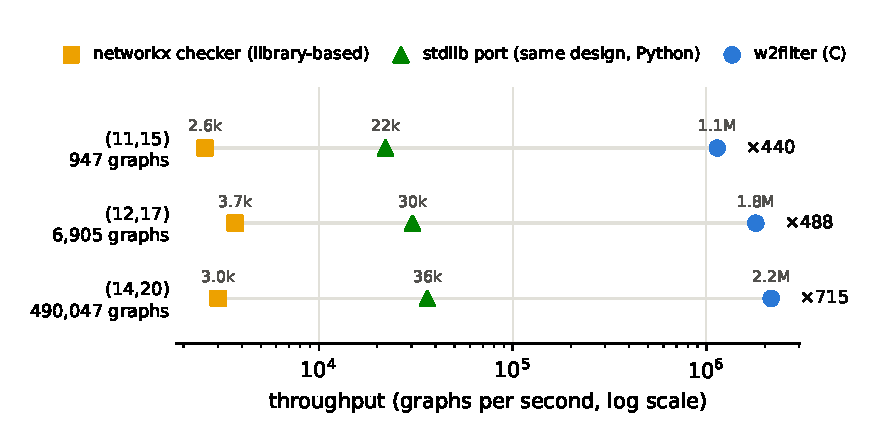
\includegraphics[width=.85\linewidth]{fig_bench}
\caption{Throughput of the three shipped implementations on the
anchor classes: single core, generation excluded, interpreter
startup subtracted (\texttt{tests/bench\_impls.py}, data shipped
as \texttt{paper/impl\_bench.csv}). The \texttt{networkx} checker
stands in for the library-based design the campaign started from;
the ratio at the right of each row is the C filter versus the
checker.}
\label{fig:bench}
\end{figure}

Single core (gcc \texttt{-O3}, commodity desktop), class
$(V,E)=(14,20)$, $490\,047$ graphs: on pre-generated input the
filter sustains $\approx 2.2\times 10^6$ graphs/s; end to end,
including generation, the pipeline takes $6.45$\,s
($\approx 7.6\times 10^4$ graphs/s), so the \texttt{geng} generator
accounts for nearly all of the wall time. Stage statistics:
back-edge kill $87.3\%$, exact stage $12.7\%$, degeneracy $0\%$,
survivors $2$. Figure~\ref{fig:bench} compares the three shipped
implementations on the anchor classes: the C filter runs
$50$--$60\times$ faster than the \texttt{stdlib} port of the same
design and $440$--$715\times$ faster than the \texttt{networkx}
checker, which stands in for the library-based approach the
campaign started from. Absolute throughputs are specific to this
machine and compiler, and the ratios also depend on the Python
environment: in an independent re-run on different hardware (a
single-vCPU cloud instance) the C throughput reproduced within
$15\%$ while the ratios compressed to $\approx 42$--$48\times$ and
$\approx 365$--$484\times$. What transfers is the order of
magnitude, tens$\times$ over the port and hundreds$\times$ over the
checker, together with the stage percentages, which are exact. Across $500$ seeded random
windows (\texttt{tests/window\_stats.sh}, data in
\texttt{paper/window\_stats.csv}) the prefilter's kill share falls
as $L_{\max}$ approaches the largest possible depth gap $n-1$ and
vanishes past it ($52\%$ of the sampled windows); the exact stage
absorbs the load in that regime, with no effect on correctness. In
production (8 workers via \texttt{geng} residue splitting,
class $(19,28)$, $\approx 10^{11}$ graphs) the generator, not the
filter, is the bottleneck.

\section{Limitations and reuse}

Vertex counts are limited to $n \le 31$ (32-bit masks); the source
documents exactly which constants to enlarge for a 64-bit port,
including the new stack bounds. The window and pair-set are
parametric (\texttt{--cycles}, \texttt{--pairset}); users replacing
the default window should check whether generator-side pre-filters
(such as \texttt{geng -f}) remain valid for their parameters, or
drop them: the exact stage re-checks every cycle length in either
case. Throughout this note ``certified'' means that every pruning
step is covered by a human-checked proof shipped with the source
(\texttt{docs/proofs.md}); the proofs are not machine-checked, and
formalising them is a natural further hardening step. Applications
beyond our campaign include cycle-spectrum--constrained
extremal problems, girth-type searches and counterexample hunts
where certified exhaustiveness matters.

\section*{Availability}

Source, proofs (\texttt{docs/proofs.md}), validation targets, CI
configuration and the benchmark data are maintained at
\url{https://github.com/Whoneon/w2filter}; version 1.0.0, described
here, is archived at
\href{https://doi.org/10.5281/zenodo.21575202}{doi:10.5281/zenodo.21575202}.
External dependency: \texttt{nauty} (B.~D. McKay) for graph
generation.

\begin{thebibliography}{9}
\bibitem{nauty} B.~D. McKay and A.~Piperno,
\emph{Practical graph isomorphism, II},
J. Symbolic Comput.\ 60 (2014), 94--112.
\bibitem{eg} P.~Erd\H{o}s,
\emph{Some old and new problems in various branches of
combinatorics}, Discrete Math.\ 165/166 (1997), 227--231.
\end{thebibliography}

\end{document}
